\documentclass{standalone}
\usepackage{pgfplots}
\usetikzlibrary{shapes.geometric, intersections, calc}
\pgfplotsset{compat=1.7}

\begin{document}
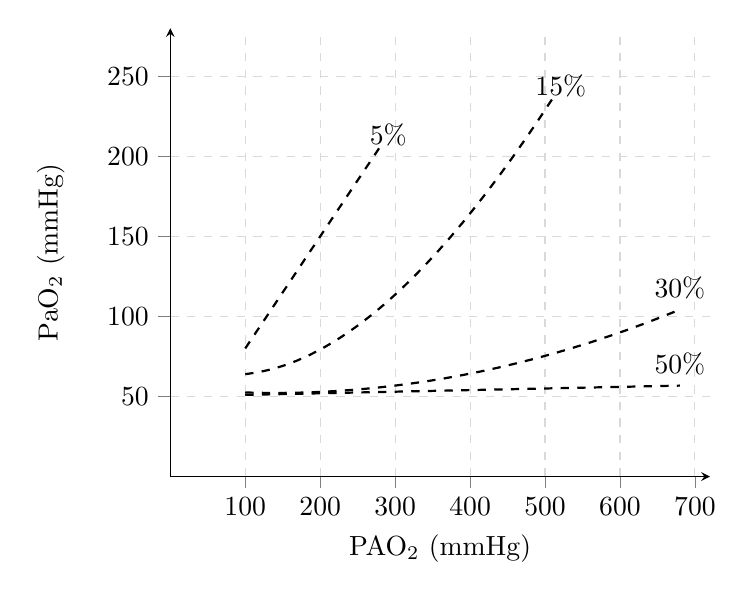
\begin{tikzpicture}[dot/.style={circle,inner sep=1pt,fill,label={#1},name=#1},
 extended line/.style={shorten >=-#1,shorten <=-#1},
 extended line/.default=10cm]

    \begin{axis}[
        axis x line=middle,
        axis y line=middle,
        grid = major,
        grid style={dashed, gray!30},
    	  x label style={at={(axis description cs:0.5,-0.1)},anchor=north},
	  y label style={at={(axis description cs:-0.1,.5)},rotate=90,anchor=south},
        xmin=0,
        xmax= 720,
        ymin= 0,
        ymax= 280,
	extra y ticks={300},
	 ylabel near ticks,
	xlabel near ticks,
        xlabel=PAO\textsubscript{2} (mmHg),
        ylabel=PaO\textsubscript{2} (mmHg),
        tick align=outside,
        enlargelimits=false]

\addplot[black,dashed,thick, domain=100:680] {50 + 0.01*x} node[black,pos=1, above]{50\%};

\addplot[black,dashed,thick, domain=100:680] {55.71429 - 0.05*x + 0.0001785714*x^2} node[black,pos=1, above]{30\%};

\addplot[black,dashed,thick, domain=100:510] {70 - 0.1761905*x + 0.001196429*x^2 - 4.166667e-7*x^3} node[black,pos=1.03]{15\%};

\addplot[black,dashed,thick, domain=100:280] {10 + 0.7*x + 0*x^2} node[black,pos=1.06]{5\%};

\end{axis}
\end{tikzpicture} 
\end{document}